%%%%%%%%%%%%%%%%%%%%%%%%%%%%%%%%%%%%%%%%%%%%%%%%%%%%%%%%%%%%%%%%%%%%%%
% LaTeX Example: Project Report
%
% Source: http://www.howtotex.com
%
% Feel free to distribute this example, but please keep the referral
% to howtotex.com
% Date: March 2011 
% 
%%%%%%%%%%%%%%%%%%%%%%%%%%%%%%%%%%%%%%%%%%%%%%%%%%%%%%%%%%%%%%%%%%%%%%
% How to use writeLaTeX: 
%
% You edit the source code here on the left, and the preview on the
% right shows you the result within a few seconds.
%
% Bookmark this page and share the URL with your co-authors. They can
% edit at the same time!
%
% You can upload figures, bibliographies, custom classes and
% styles using the files menu.
%
% If you're new to LaTeX, the wikibook is a great place to start:
% http://en.wikibooks.org/wiki/LaTeX
%
%%%%%%%%%%%%%%%%%%%%%%%%%%%%%%%%%%%%%%%%%%%%%%%%%%%%%%%%%%%%%%%%%%%%%%
% Edit the title below to update the display in My Documents
%\title{Project Report}
%
%%% Preamble
\documentclass[paper=a4, fontsize=11pt]{scrartcl}
\usepackage[T1]{fontenc}
\usepackage{fourier}

\usepackage[english]{babel}															% English language/hyphenation
\usepackage[protrusion=true,expansion=true]{microtype}	
\usepackage{amsmath,amsfonts,amsthm} % Math packages
\usepackage[pdftex]{graphicx}	
\usepackage{url}
\graphicspath{ {report/} }


%%% Custom sectioning
\usepackage{sectsty}
\allsectionsfont{\centering \normalfont\scshape}


%%% Custom headers/footers (fancyhdr package)
\usepackage{fancyhdr}
\pagestyle{fancyplain}
\fancyhead{}											% No page header
\fancyfoot[L]{}											% Empty 
\fancyfoot[C]{}											% Empty
\fancyfoot[R]{\thepage}									% Pagenumbering
\renewcommand{\headrulewidth}{0pt}			% Remove header underlines
\renewcommand{\footrulewidth}{0pt}				% Remove footer underlines
\setlength{\headheight}{13.6pt}


%%% Equation and float numbering
\numberwithin{equation}{section}		% Equationnumbering: section.eq#
\numberwithin{figure}{section}			% Figurenumbering: section.fig#
\numberwithin{table}{section}				% Tablenumbering: section.tab#


%%% Maketitle metadata
\newcommand{\horrule}[1]{\rule{\linewidth}{#1}} 	% Horizontal rule

\title{
		%\vspace{-1in} 	
		\usefont{OT1}{bch}{b}{n}
		%\normalfont \normalsize \textsc{School of random department names} \\ [25pt]
		\horrule{0.5pt} \\[0.4cm]
		\huge Government of India Hackathon: Medical Expert Search Engine technical report and documentation\\
		\horrule{2pt} \\[0.5cm]
}
\author{
		\normalfont 								\normalsize
        Wei Wang, Yash Pratyush Sinha\\[-3pt]		\normalsize
        \today
}
\date{}


%%% Begin document
\begin{document}
\maketitle
\section{Aim}
A tool for Mining MEDLINE/Pubmed for identifying subject Experts. Mediline/Pubmed is an xml based repository of medical papers and their authors and abstracts. Our tool must mine it, and should give a ranked list of experts based on a search query.


\section{Requirements}
We have two major requirements:
\begin{itemize}
\item Pubmed\/Medline data containing at least the paper, it's references it', it's Medical Subject headings (MeSH) \& keywords and it's author's names.
\item A big medical knowledge graph, similar to wordnet (or babelnet) so as to search and understand the medical search terms much more effectively. 
Since our extensive search did not let us find any freely available medical wornet, we built our own solution to find similar words using tf-idf.
\end{itemize}

\subsection{Technology}
Python, with scikit-learn and pandas for most of the searching, and heavy lifting. \\
R for some of the parsing.\\
MySQL for database.\\
Php for the web application \\

%\begin{align}
%	A = 
%	\begin{bmatrix}
%	A_{11} & A_{21} \\
%  	A_{21} & A_{22}
%	\end{bmatrix}
%\end{align}

\section{Algortihms}
We have used several algorithms in our project. They are:
\subsection{Z-Score}
Z-score is a method of scoring a particular author according to how many papers has he/she written about that given subject.
For this, we first define a few variables:
\begin{center}
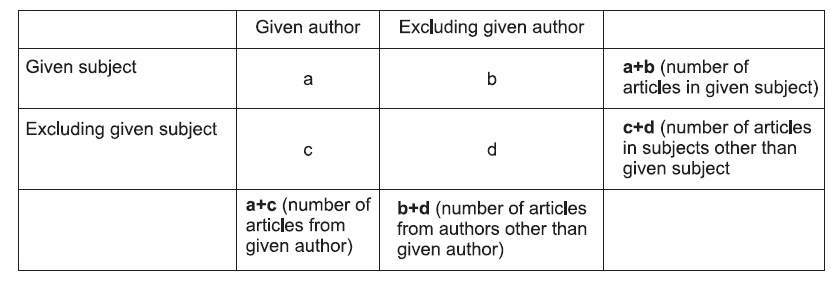
\includegraphics[scale=0.75]{zscorematrix}
\end{center}
Using these variables, we define the algorithm as follows: 
\begin{center}
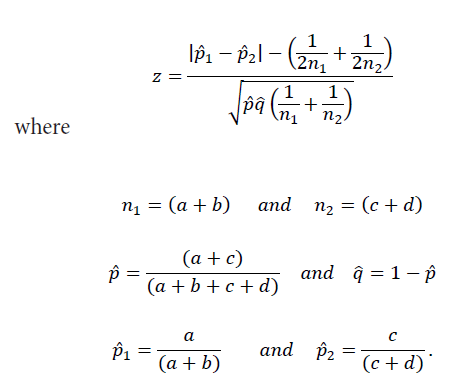
\includegraphics[scale=0.85]{ascoreformula}
\end{center}
Now, this z-score increases with higher number of papers in the given field, decreases with diversity and increases with specialization. For more informations, refer to \cite{zscore}

\subsection{Pagerank}
\begin{center}
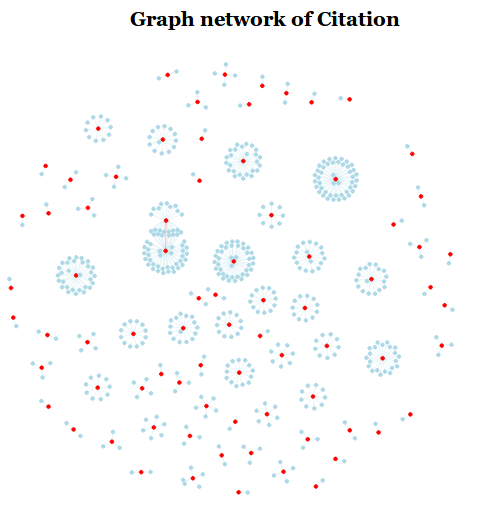
\includegraphics[scale=0.55]{citation_graph} \\
\end{center}

We have used Google's pagerank algorithm to devlope a ranking system of all papers where each paper cites another paper. This way we can set papers which have been cited more as more important. For more information about pagerank, refer to \cite{prank}

\subsection{FLAE}
FLAE or First-Last Author Emphasis is a simple algorthim using which one can score individual author for a given paper. In this, the first author should get credit of the whole impact, the last author half, and the credit of the other authors is the impact divided by the number of all authors. For more information, refer to \cite{flae}.

\subsection{Medical Dictionary to Term Similarity builder}
This is an in-house developed algorithm which given a list of medical terms and their definitions, can use these definitions to find terms simliar to the one given in query. This is done by assuming each term-definition as a separate document and then calculating the tf-idf for each word in each document/definition. It then multiplies the tf-idf score of common words of each definition to find the similarity between them. By thresholding this similarity score at $0.25$, we can say whether two terms are similar or not

\section{Overall Method}
\begin{enumerate}
\item On getting a search term, we find similar term to the given query. We call this list as $T$.
\item We search all papers with any word of $T$ in their MeSH or Keywords. Each paper is given a 'relevance score' according to how many terms of $T$ are present in it. Using these papers, we built a set of authors $A$ which has to be ranked
\item We calculate weighted $a$,$b$,$c$ and $d$ (as in z-score) for each author, where every number of paper is multiplied by the relevance score and it's page rank score.
\item We calculate this weighted z-score for each author and rank them according to it.
\end{enumerate}

%
%\paragraph{Heading on level 4 (paragraph)}
%Lorem ipsum dolor sit amet, consectetuer adipiscing elit. Aenean commodo ligula eget dolor. Aenean massa. Cum sociis natoque penatibus et magnis dis parturient montes, nascetur ridiculus mus. Donec quam felis, ultricies nec, pellentesque eu, pretium quis, sem. Nulla consequat massa quis enim. 

\begin{thebibliography}{9}

\bibitem{zscore} {Developing a Biomedical Expert Finding System
Using Medical Subject Headings, Harpreet Singh, PhD, Reema Singh, PhD, Arjun Malhotra, MSc, Manjit Kaur, MCA http://dx.doi.org/10.4258/hir.2013.19.4.243}

\bibitem{prank} {A Document Clustering and Ranking System for Exploring
MEDLINE Citations, YONGJING LIN , Ms, WENYUAN LI , PHD, KEKE CHEN , PHD, YING LIU , PHD Journal of the American Medical Informatics Association Volume 14 Number 5 Sept / Oct 2007 }

\bibitem{flae} {Author Sequence and Credit for Contributions in Multiauthored Publication, Teja Tscharntke, Michael E Hochberg, Tatyana A Rand, Vincent H Resh, and Jochen Krauss doi:10.1371/journal.pbio.0050018}

\end{thebibliography}

\end{document}
